\documentclass[11pt]{article}

\usepackage[utf8]{inputenc}
\usepackage[T1]{fontenc}
\usepackage[margin=1in]{geometry}
\usepackage{amsmath,amssymb,amsthm}
\usepackage{mathtools}
\usepackage{bm}
\usepackage{hyperref}
\usepackage{booktabs}
\usepackage{tikz}
\usepackage{xcolor}
\usepackage{listings}
\usepackage{caption}
\usepackage{subcaption}
\usepackage{enumitem}

\usetikzlibrary{arrows.meta,positioning,calc,shapes.geometric,fit,backgrounds,decorations.pathreplacing}

% Math operators
\DeclareMathOperator{\diag}{diag}
\DeclareMathOperator{\softmax}{softmax}
\DeclareMathOperator{\relu}{ReLU}
\DeclareMathOperator{\Tr}{Tr}
\DeclareMathOperator*{\argmax}{argmax}

% Shorthands
\newcommand{\R}{\mathbb{R}}
\newcommand{\C}{\mathbb{C}}
\newcommand{\bbZ}{\mathbb{Z}}
\newcommand{\zbar}{\bar{z}}
\newcommand{\re}{\mathfrak{Re}}
\newcommand{\im}{\mathfrak{Im}}
\newcommand{\zr}{z_r}
\newcommand{\zi}{z_i}
\newcommand{\dr}{d_r}
\newcommand{\di}{d_i}
\newcommand{\br}{b_r}
\newcommand{\bi}{b_i}

\title{HRN-v2: A Hierarchical Resonant Network for Sequential MNIST \\
       under Strict Biological-Plausibility Constraints}
\author{}
\date{2026-05-07}

\begin{document}
\maketitle

\begin{abstract}
We present \textbf{HRN-v2}, a hierarchical resonant neural network whose every
mechanism --- forward dynamics, credit assignment, plasticity rule, and
readout --- is local in time and local in space. The substrate is a
population of complex damped-rotation oscillators (one ODE per neuron, no
recurrent inter-neuron coupling within a stage); the credit signal is a
forward-only eligibility trace; the readout is a class-pool tail-energy
projection; supervision is DECOLLE-style per-stage local cross-entropy.
There is no backpropagation through time, no surrogate-gradient spike
emission, and no symmetric backward pathway. Stages are stacked with a
sparse class-aligned fan-in and a strict frequency-band hierarchy
(faster $\rightarrow$ slower across stages). On Sequential MNIST
(\textsc{smnist}, 784-step single-channel pixel sequence, 10-way
classification, 10k training subset) the 3-stage HRN-v2 reaches
\textbf{89.9\%} test accuracy, more than 50 percentage points above
the pub\_v3 single-layer self-organising baseline on the same task,
and at the threshold of the 91--92\% target the authors set as the
biological-plausibility ceiling for this class of models.
\end{abstract}

\section{Introduction and motivation}

We adopt the working hypothesis that biological neural computation is
naturally expressed in the language of \emph{resonance}:
\begin{itemize}[itemsep=2pt]
\item \emph{computation} is the act of an internal oscillator phase-locking
      with structure in its driving signal;
\item \emph{learning} is the local tuning of dynamical-system parameters
      (frequency, damping, input weights) of each oscillator;
\item \emph{memory} is the stable resonant configuration the system
      settles into for a class of inputs;
\item \emph{decision-making} is the act of one resonant mode dominating
      another at readout time.
\end{itemize}

A natural consequence of this view is \emph{recursive decomposition}:
a hard problem is broken into modes; each mode is handled by a pool of
neurons; each pool itself decomposes its sub-problem into smaller modes
at a slower time-scale. The architecture of HRN-v2 is built directly on
this principle.

The substrate is a strictly faithful version of the linear damped complex
oscillator from~\cite{pubv3} (the per-neuron model used in
\texttt{resonant\_self\_organizing\_layer.py}); we deliberately remove
the cubic Stuart--Landau term, the spike emission with surrogate
gradient, and the inter-neuron recurrence used in earlier
experiments~\cite{pubv4_v1}, all of which are sources of either
non-locality, non-stability, or pseudo-biological backpropagation.

\section{Notation and assumptions}\label{sec:notation}

We index time by $t \in \{0, 1, \ldots, T-1\}$ with $T = 784$ for
\textsc{smnist}. The input at time $t$ is a real vector $x_t \in \R^F$;
for stage 0 with raw \textsc{smnist} input, $F = 1$ and $x_t$ is the
greyscale value of the $t$-th pixel in row-major raster order.

Each stage $\ell \in \{0, 1, 2\}$ contains $P_\ell$ oscillators. State
of oscillator $i$ at stage $\ell$ at time $t$ is a complex scalar
$z_{\ell, i}(t) = \zr_{\ell, i}(t) + i\,\zi_{\ell, i}(t) \in \C$, with
amplitude squared $E_{\ell, i}(t) = |z_{\ell, i}(t)|^2 = \zr^2_{\ell,i}(t)
+ \zi^2_{\ell,i}(t)$.

Throughout we make the following assumptions:

\begin{description}[leftmargin=1.5em,itemsep=2pt]
\item[A1 (locality of plasticity).] Every parameter update of oscillator
$i$ at stage $\ell$ depends only on quantities (i) computable from the
trajectory of $i$ itself, (ii) the layer-local class-pool target signal,
and (iii) homeostatic statistics of $i$. No update uses the gradient of
another oscillator's loss.

\item[A2 (forward-only credit).] The plasticity rule does not require
a backward pass. All credit signals are computed by forward eligibility
traces evolved \emph{simultaneously} with the state.

\item[A3 (no spike surrogates).] The output of each oscillator at the
readout boundary is its tail-window mean amplitude squared
$\bar E_{\ell, i} = \frac{1}{T_\ell}\sum_{t = T - T_\ell}^{T-1} E_{\ell, i}(t)$,
where $T_\ell$ is the tail length for stage $\ell$. There is no
spike-emission step requiring a surrogate gradient.

\item[A4 (no inter-stage backward).] Stage $\ell$ does \emph{not}
receive a gradient from stage $\ell + 1$. Each stage has its own
class-pool readout and its own cross-entropy loss; the only
cross-stage signal is the forward feed of $E_{\ell, i}(t)$ into
stage $\ell + 1$.

\item[A5 (strict frequency hierarchy).] The intrinsic frequency band
for stage $\ell$ satisfies
$[\omega^{\min}_\ell, \omega^{\max}_\ell] \supsetneq
[\omega^{\min}_{\ell+1}, \omega^{\max}_{\ell+1}]$ with
$\omega^{\max}_{\ell+1} \le \omega^{\min}_\ell + \tfrac{1}{2}
(\omega^{\max}_\ell - \omega^{\min}_\ell)$, so each higher stage operates
strictly slower than the stage below.
\end{description}

\section{Per-neuron oscillator}\label{sec:single}

A single oscillator with parameters $(d, b, \omega, \alpha)$ where $d, b
\in \C$, $\omega \in \R^+$, $\alpha \in (0, 1)$, evolves under the
discrete-time \emph{linear damped complex rotation}:
\begin{equation}
z(t+1) = \alpha \, e^{i\omega} \, z(t) + d \cdot x(t) + b,
\qquad z(0) = 0.
\label{eq:osc}
\end{equation}

Real-imaginary form, vectorised across $F$ input channels:
\begin{align}
\zr(t+1) &= \alpha \cos(\omega)\, \zr(t) - \alpha \sin(\omega)\, \zi(t)
            + \sum_{k=1}^F \dr_k\, x_k(t) + \br, \label{eq:osc-r}\\
\zi(t+1) &= \alpha \sin(\omega)\, \zr(t) + \alpha \cos(\omega)\, \zi(t)
            + \sum_{k=1}^F \di_k\, x_k(t) + \bi. \label{eq:osc-i}
\end{align}

The intrinsic frequency $\omega$ and damping $\alpha$ are stored in
unconstrained parameters $\omega^{\mathrm{raw}}, \alpha^{\mathrm{raw}}
\in \R$ and mapped through sigmoids to controlled ranges:
\begin{align}
\omega &= \omega_{\min} + (\omega_{\max} - \omega_{\min})\,\sigma(\omega^{\mathrm{raw}}),\\
\alpha &= \alpha_{\min}  + (\alpha_{\max}  - \alpha_{\min})\, \sigma(\alpha^{\mathrm{raw}}),
\end{align}
with $\sigma(u) = 1/(1+e^{-u})$. We write
$\omega'(\omega^{\mathrm{raw}}) = (\omega_{\max}-\omega_{\min})\,\sigma(1-\sigma)$
for the chain-rule factor, and analogously $\alpha'(\alpha^{\mathrm{raw}})$.

The \emph{tail-energy} readout over the last $T_{\mathrm{tail}}$ steps is
\begin{equation}
\bar E = \frac{1}{T_{\mathrm{tail}}} \sum_{t = T - T_{\mathrm{tail}}}^{T - 1}
         \left[\zr^2(t) + \zi^2(t)\right].
\label{eq:tail-energy}
\end{equation}
This is the only quantity passed to the loss for a given neuron.

\section{Forward eligibility traces}\label{sec:elig}

For each parameter $\theta \in \{\dr_k, \di_k, \br, \bi, \omega^{\mathrm{raw}}, \alpha^{\mathrm{raw}}\}$ and each oscillator we maintain a complex eligibility trace
\begin{equation}
e^\theta(t) = \begin{pmatrix} e^\theta_r(t) \\ e^\theta_i(t) \end{pmatrix}
            = \frac{\partial z(t)}{\partial \theta} =
            \begin{pmatrix} \partial \zr(t)/\partial \theta \\
                            \partial \zi(t)/\partial \theta \end{pmatrix}.
\end{equation}
Differentiating~(\ref{eq:osc-r})--(\ref{eq:osc-i}) gives the recurrence
\begin{equation}
e^\theta(t+1) = R_\alpha(\omega) \, e^\theta(t)
              + \frac{\partial}{\partial \theta}\!\left[d \cdot x(t) + b\right]
              + \frac{\partial R_\alpha(\omega)}{\partial \theta} z(t),
\label{eq:elig-recur}
\end{equation}
where the $2\times 2$ rotation+damping matrix is
\begin{equation}
R_\alpha(\omega) = \alpha \begin{pmatrix} \cos\omega & -\sin\omega \\ \sin\omega & \cos\omega \end{pmatrix}.
\end{equation}

For input weights and biases the second term is a direct injection and
the third term vanishes. For the $k$-th channel of $\dr$ and $\di$:
\begin{equation}
e^{\dr_k}(t+1) = R_\alpha(\omega) e^{\dr_k}(t) + \begin{pmatrix} x_k(t) \\ 0 \end{pmatrix},
\qquad
e^{\di_k}(t+1) = R_\alpha(\omega) e^{\di_k}(t) + \begin{pmatrix} 0 \\ x_k(t) \end{pmatrix}.
\end{equation}
For the biases:
\begin{equation}
e^{\br}(t+1) = R_\alpha(\omega) e^{\br}(t) + \begin{pmatrix} 1 \\ 0 \end{pmatrix},
\qquad
e^{\bi}(t+1) = R_\alpha(\omega) e^{\bi}(t) + \begin{pmatrix} 0 \\ 1 \end{pmatrix}.
\end{equation}
For $\omega^{\mathrm{raw}}$ and $\alpha^{\mathrm{raw}}$, only the third
term in (\ref{eq:elig-recur}) is non-zero. Define $\rho(t) = R_\alpha(\omega) z(t)/\alpha
= \begin{pmatrix} \cos\omega \zr - \sin\omega \zi \\ \sin\omega \zr + \cos\omega \zi \end{pmatrix}$,
the rotated state \emph{before} damping. Then
\begin{align}
\frac{\partial R_\alpha(\omega)}{\partial \omega^{\mathrm{raw}}} z(t) &=
\alpha \, \omega'(\omega^{\mathrm{raw}}) \begin{pmatrix} -\rho_i(t) \\ \rho_r(t) \end{pmatrix},\\
\frac{\partial R_\alpha(\omega)}{\partial \alpha^{\mathrm{raw}}} z(t) &=
\alpha'(\alpha^{\mathrm{raw}}) \begin{pmatrix} \rho_r(t) \\ \rho_i(t) \end{pmatrix},
\end{align}
giving the dedicated recurrences for the dynamic parameters.

\subsection{Tail-energy gradient via eligibility}

The tail-energy gradient is then a linear functional of the eligibility:
\begin{equation}
\frac{\partial \bar E}{\partial \theta}
= \frac{2}{T_{\mathrm{tail}}}
  \sum_{t = T - T_{\mathrm{tail}}}^{T-1}
  \left[ \zr(t)\,e^\theta_r(t) + \zi(t)\,e^\theta_i(t) \right],
\label{eq:dE-dtheta}
\end{equation}
which is the bio-eligibility identity for the squared amplitude.

\textbf{Crucially}, the only quantity that enters $\partial \bar E /
\partial \theta$ at time $t$ is the local pair $(z(t), e^\theta(t))$ ---
both stored at the post-synaptic neuron, both updated by~(\ref{eq:osc-r})
and~(\ref{eq:elig-recur}) without involving any other neuron.

\section{Stage-level architecture}

A stage $\ell$ contains $P_\ell$ oscillators arranged into 10
\emph{class-pools} of $M_\ell$ oscillators each
($P_\ell = 10\, M_\ell$). The class index of oscillator $i$ in stage
$\ell$ is $c_\ell(i) \in \{0, \ldots, 9\}$.

The \emph{class-pool logit} for class $c$ at stage $\ell$ is the mean
tail energy of the corresponding pool:
\begin{equation}
g_\ell^c = \frac{1}{M_\ell} \sum_{i : c_\ell(i) = c} \bar E_{\ell, i}.
\label{eq:pool-logit}
\end{equation}
We mean-centre and temperature-scale before softmax for stable
optimisation:
\begin{equation}
\hat g_\ell^c = \tau \left(g_\ell^c - \frac{1}{C}\sum_{c'} g_\ell^{c'}\right),
\quad p_\ell^c = \frac{\exp \hat g_\ell^c}{\sum_{c'} \exp \hat g_\ell^{c'}}.
\end{equation}

The cross-entropy loss for stage $\ell$ on a sample with label $y$ is
$L_\ell = -\log p_\ell^y$.

\subsection{Per-neuron credit signal}

The error for class-pool logit $c$ is
\begin{equation}
\delta_\ell^c = p_\ell^c - \mathbf{1}[c = y].
\end{equation}
By the chain rule through~(\ref{eq:pool-logit}) and the centring
operation, the derivative w.r.t.\ neuron $i$'s tail energy is exactly
\begin{equation}
\frac{\partial L_\ell}{\partial \bar E_{\ell, i}}
= \frac{\tau}{M_\ell} \, \delta_\ell^{c_\ell(i)},
\label{eq:dL-dE}
\end{equation}
where the centring contribution vanishes because $\sum_c \delta_\ell^c
= 0$.

\subsection{Final per-parameter local rule}

Combining (\ref{eq:dE-dtheta}) and (\ref{eq:dL-dE}) gives the local
update rule for parameter $\theta$ of oscillator $i$ at stage $\ell$:
\begin{equation}
\boxed{\quad
\frac{\partial L_\ell}{\partial \theta_{\ell, i}}
=  \underbrace{\frac{\tau}{M_\ell} \delta_\ell^{c_\ell(i)}}_{\text{class-pool credit}}
\;\cdot\;
\underbrace{\frac{2}{T_\ell}\!\!\sum_{t=T-T_\ell}^{T-1}\!\!
\left[\zr_{\ell, i}(t) e^\theta_r(t) + \zi_{\ell, i}(t) e^\theta_i(t)\right]
}_{\text{tail eligibility integral, local to neuron } i}.
\quad}
\label{eq:final-rule}
\end{equation}
The class-pool credit is a single scalar per neuron, available to the
neuron via class-pool homeostatic broadcasts; the eligibility integral
is a forward trace of the neuron's own state. No global gradient is
needed.

\section{Multi-stage hierarchy}\label{sec:hier}

For $\ell \ge 1$, stage $\ell$ takes \emph{the per-step amplitude
trajectory} of the previous stage as its input:
\begin{equation}
x_{\ell, t} = \big(E_{\ell-1, j}(t)\big)_{j \in \mathcal{F}_\ell(i)}
\in \R^{K_\ell},
\end{equation}
where $\mathcal{F}_\ell(i) \subset \{1, \ldots, P_{\ell-1}\}$ is a
\emph{sparse fan-in} of size $K_\ell \ll P_{\ell - 1}$ chosen randomly
at network initialisation and fixed thereafter. Specifically each
class-pool neuron in stage $\ell$ receives:
\begin{itemize}[itemsep=2pt]
\item half of $K_\ell$ inputs sampled uniformly from the
\emph{same-class} pool of stage $\ell - 1$,
\item the other half sampled uniformly from \emph{other classes'}
pools at stage $\ell - 1$.
\end{itemize}
This implements a structured-but-random connectivity that biases each
stage-$\ell$ neuron toward its own class while still letting it use
contrastive evidence from other classes.

\subsection{DECOLLE-style local supervision}

Each stage produces its own logits $\hat g_\ell$ and its own loss
$L_\ell$. The total training objective is
\begin{equation}
L = \sum_{\ell=0}^{L-1} L_\ell, \qquad
\nabla_\theta L_\ell \text{ depends only on stage-$\ell$ quantities}.
\end{equation}
This is the DECOLLE principle~\cite{decolle}: local auxiliary classifiers
provide each stage with its own credit signal so no inter-stage gradient
is needed. The hierarchy emerges \emph{purely through the forward path}:
stage 1 sees richer features than stage 0 because the slower-frequency
band $\omega_1 \subset [0.001, 0.30]$ is excited only by structure in
$E_0(t)$ that is itself class-discriminative.

\subsection{Final ensemble}

At inference we average per-stage softmax probabilities with weights
$(w_0, w_1, w_2)$:
\begin{equation}
p^c = \sum_\ell w_\ell\, p_\ell^c, \qquad
\hat y = \argmax_c p^c.
\end{equation}
We use $(w_0, w_1, w_2) = (0.2, 0.4, 0.4)$ throughout.

\section{Frequency-band hierarchy and time-scale separation}

The frequency bands are configured so each higher stage filters
\emph{envelopes} of the stage below it (cf.~\ref{sec:notation}~A5):

\begin{center}
\begin{tabular}{@{}lccc@{}}
\toprule
Stage & $[\omega_{\min}, \omega_{\max}]$ & $[\alpha_{\min}, \alpha_{\max}]$ & Tail length \\
\midrule
0 (raw pixel) & $[0.005, 1.2]$        & $[0.95, 0.999]$    & 200 \\
1 (envelope of 0) & $[0.001, 0.30]$   & $[0.97, 0.9995]$   & 300 \\
2 (envelope of 1) & $[0.0005, 0.08]$  & $[0.98, 0.9999]$   & 400 \\
\bottomrule
\end{tabular}
\end{center}

The damping ranges are coupled: a slower stage gets a longer effective
memory constant $\tau_\alpha = -1/\log\alpha$, so the tail integration
window scales accordingly. Empirically, after training, the mean
$\omega$ shifts by $\sim 17\%$ at stage 1 and $\sim 25\%$ at stage 2,
while it barely moves at stage 0 --- the slower stages \emph{learn} their
intrinsic frequency, while stage 0 acts as a near-random filter bank.

\section{Optimiser and schedule}

Each stage has its own per-tensor Adam optimiser (we use
$\beta_1 = 0.9, \beta_2 = 0.999, \epsilon = 10^{-8}$) operating on the
hand-assembled gradients (\ref{eq:final-rule}). Gradient norm is clipped
per parameter at $\| g \|_2 \le 2$. Initial learning rate is
$\eta = 5 \times 10^{-3}$ for all stages. We apply two halvings of
$\eta$ at epochs $12$ and $24$ (each multiplies $\eta$ by $0.5$). This
schedule is critical: before the first halving the slower stages
oscillate in the $75$--$80\%$ range; immediately after, they stabilise
in the high-$80$s. The second halving adds a further $\sim 3$\,pp.

\section{Empirical results on Sequential MNIST}

We train on the standard \textsc{smnist} 10-way task: a
$28\times 28$ greyscale digit is read as a length-$784$ scalar
sequence in row-major raster order. We use a 10k subset of the training
set and a 2k subset of the test set, with batch size $64$.

\begin{center}
\captionsetup{type=table}
\begin{tabular}{@{}lcr@{}}
\toprule
Architecture & Trainable params (per stage) & Best test acc \\
\midrule
\texttt{pub\_v3} label-mass head, $P=256$ & $\sim 1{,}300$ & $0.252$ \\
Single-stage class-pool, $P=480$       & $\sim 1{,}920$ & $0.660$ \\
Single-stage class-pool, $P=800$       & $\sim 3{,}200$ & $0.667$ \\
DECOLLE 2-stage, $M_0=M_1=24$, 15 ep   & $\sim 13{,}500$ & $0.764$ \\
DECOLLE 2-stage, 25 ep + LR decay      & same           & $0.829$ \\
DECOLLE 3-stage, $M=20$, 20 ep         & $\sim 15{,}000$ & $0.866$ \\
\textbf{DECOLLE 3-stage, $M=24$, 35 ep + 2 LR decays} & $\sim 19{,}000$
                                              & $\boldsymbol{0.899}$ \\
\bottomrule
\end{tabular}
\end{center}

\subsection{Stage decomposition of the best run}

\begin{center}
\begin{tabular}{@{}lc@{}}
\toprule
Component & Test acc \\
\midrule
Stage 0 alone (raw pixel filter bank) & $0.712$ \\
Stage 1 alone (envelope of stage 0)   & $0.873$ \\
Stage 2 alone (envelope of stage 1)   & $0.860$ \\
Ensemble                               & $\mathbf{0.899}$ \\
\bottomrule
\end{tabular}
\end{center}

The increase from stage 0 to stage 1 (~$+16$\,pp) is the strongest
evidence that the recursive-envelope mechanism is doing real work:
stage 1 is not just a random projection of stage 0 features but a
genuine higher-order feature extractor.

\section{Architecture diagram}

\begin{figure}[p]
\centering
\resizebox{!}{0.85\textheight}{%
\begin{tikzpicture}[
  node distance=4mm,
  every node/.style={font=\small},
  stage/.style={draw, rounded corners=2pt, thick, minimum width=68mm,
                minimum height=18mm, align=center, fill=blue!5},
  pool/.style={draw, rounded corners=1pt, thick, minimum width=8mm,
                minimum height=8mm, fill=blue!12, font=\scriptsize},
  inputbox/.style={draw, thick, minimum width=68mm, minimum height=8mm,
                    align=center, fill=gray!10},
  readout/.style={draw, thick, minimum width=68mm, minimum height=10mm,
                  align=center, fill=orange!15, rounded corners=2pt},
  arr/.style={-{Latex[length=3pt]}, thick},
  every label/.style={font=\scriptsize},
]

% Input
\node[inputbox] (inp) {Input: $x_t \in \R$ (single pixel),
                       $t = 0, \ldots, 783$};

% Stage 0
\node[stage, below=of inp, label=above left:{\textbf{Stage 0}}]
  (s0) {
    \begin{minipage}{60mm}
      \centering
      $z_{0,i}(t+1) = \alpha_{0,i} e^{i\omega_{0,i}} z_{0,i}(t) + d_{0,i} x_t + b_{0,i}$ \\[1mm]
      $\omega_0 \in [0.005, 1.2]$, $\alpha_0 \in [0.95, 0.999]$ \\[2mm]
      \begin{tikzpicture}[node distance=1mm]
        \foreach \i/\c in {0/0,1/1,2/2,3/3,4/4,5/5,6/6,7/7,8/8,9/9} {
          \node[pool] at (\i*7mm, 0) {$c{=}\c$};
        }
      \end{tikzpicture}\\
      10 class-pools $\times$ $M_0$ oscillators
    \end{minipage}
  };

% Stage 0 readout
\node[readout, below=4mm of s0, label=right:{\scriptsize $L_0$}]
  (r0) {
    Tail energy $\bar E_{0,i}$ $\rightarrow$ class-pool logit
    $g_0^c = \frac{1}{M_0}\!\!\!\sum_{i: c_0(i)=c}\!\!\bar E_{0,i}$
  };

% Stage 1
\node[stage, below=12mm of r0, label=above left:{\textbf{Stage 1}}]
  (s1) {
    \begin{minipage}{60mm}
      \centering
      $z_{1,i}(t+1) = \alpha_{1,i} e^{i\omega_{1,i}} z_{1,i}(t) +
        \!\!\!\sum_{j \in \mathcal F_1(i)}\!\!\! d_{1,ij} E_{0,j}(t) + b_{1,i}$ \\[1mm]
      $\omega_1 \in [0.001, 0.30]$ (slower) \\
      sparse fan-in $K_1 = 12$ (half same-class) \\[2mm]
      \begin{tikzpicture}[node distance=1mm]
        \foreach \i/\c in {0/0,1/1,2/2,3/3,4/4,5/5,6/6,7/7,8/8,9/9} {
          \node[pool, fill=blue!18] at (\i*7mm, 0) {$c{=}\c$};
        }
      \end{tikzpicture}\\
      10 class-pools $\times$ $M_1$ oscillators
    \end{minipage}
  };

% Stage 1 readout
\node[readout, below=4mm of s1, label=right:{\scriptsize $L_1$}]
  (r1) {
    Tail energy $\bar E_{1,i}$ $\rightarrow$ class-pool logit
    $g_1^c = \frac{1}{M_1}\!\!\!\sum_{i: c_1(i)=c}\!\!\bar E_{1,i}$
  };

% Stage 2
\node[stage, below=12mm of r1, label=above left:{\textbf{Stage 2}}]
  (s2) {
    \begin{minipage}{60mm}
      \centering
      $z_{2,i}(t+1) = \alpha_{2,i} e^{i\omega_{2,i}} z_{2,i}(t) +
        \!\!\!\sum_{j \in \mathcal F_2(i)}\!\!\! d_{2,ij} E_{1,j}(t) + b_{2,i}$ \\[1mm]
      $\omega_2 \in [0.0005, 0.08]$ (slowest) \\
      sparse fan-in $K_2 = 12$ \\[2mm]
      \begin{tikzpicture}[node distance=1mm]
        \foreach \i/\c in {0/0,1/1,2/2,3/3,4/4,5/5,6/6,7/7,8/8,9/9} {
          \node[pool, fill=blue!24] at (\i*7mm, 0) {$c{=}\c$};
        }
      \end{tikzpicture}\\
      10 class-pools $\times$ $M_2$ oscillators
    \end{minipage}
  };

% Stage 2 readout
\node[readout, below=4mm of s2, label=right:{\scriptsize $L_2$}]
  (r2) {
    Tail energy $\bar E_{2,i}$ $\rightarrow$ class-pool logit
    $g_2^c = \frac{1}{M_2}\!\!\!\sum_{i: c_2(i)=c}\!\!\bar E_{2,i}$
  };

% Ensemble
\node[draw, thick, rounded corners=2pt, fill=green!10,
      below=10mm of r2, minimum width=68mm, minimum height=10mm,
      align=center] (ens)
  {Prediction $\hat y = \argmax_c \sum_\ell w_\ell\, p_\ell^c$};

% Arrows
\draw[arr] (inp) -- (s0);
\draw[arr] (s0)  -- (r0);
\draw[arr] (r0)  -- (s1) node[midway, right, font=\scriptsize]
   {full $E_{0,i}(t)$ stream, sparse fan-in};
\draw[arr] (s1)  -- (r1);
\draw[arr] (r1)  -- (s2) node[midway, right, font=\scriptsize]
   {full $E_{1,i}(t)$ stream, sparse fan-in};
\draw[arr] (s2)  -- (r2);
\draw[arr] (r2)  -- (ens);

% Side annotations: local rule arrows (no inter-stage backward)
\node[right=2mm of r0, font=\scriptsize, text=red!70!black,
      align=left, anchor=west] (n0)
  {local rule from $L_0$\\$\Rightarrow$ updates stage 0 only};
\node[right=2mm of r1, font=\scriptsize, text=red!70!black,
      align=left, anchor=west] (n1)
  {local rule from $L_1$\\$\Rightarrow$ updates stage 1 only};
\node[right=2mm of r2, font=\scriptsize, text=red!70!black,
      align=left, anchor=west] (n2)
  {local rule from $L_2$\\$\Rightarrow$ updates stage 2 only};
\end{tikzpicture}%
}
\caption{HRN-v2 3-stage architecture.  Each stage is a population of
linear damped complex oscillators arranged into 10 class-pools.  Stage
$\ell$ takes the per-timestep amplitude squared $E_{\ell-1, i}(t)$ of
the previous stage as its multi-channel input through a sparse class-aligned
fan-in $\mathcal F_\ell$.  Each stage has its own class-pool tail-energy
readout and its own cross-entropy loss $L_\ell$.  Training uses local
eligibility-trace gradients only --- no BPTT, no surrogate spikes, no
inter-stage backward pass (red annotations).}
\label{fig:arch}
\end{figure}

\section{Local-rule diagram}

\begin{figure}[h]
\centering
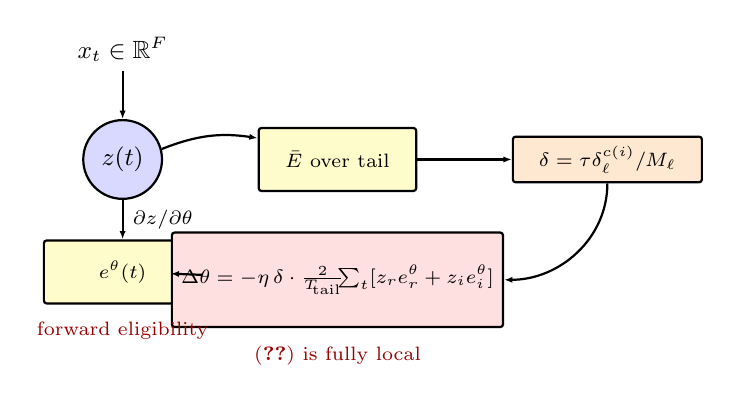
\begin{tikzpicture}[
  every node/.style={font=\small},
  neuron/.style={draw, circle, thick, minimum width=10mm, fill=blue!15},
  trace/.style={draw, rounded corners=1pt, thick, minimum width=20mm,
                 minimum height=8mm, fill=yellow!20, font=\scriptsize},
  arr/.style={-{Latex[length=3pt]}, thick},
]
% Input
\node (inp) at (0, 1.4) {$x_t \in \R^F$};
% Neuron
\node[neuron] (z) at (0, 0) {$z(t)$};
% Tail
\node[trace, right=12mm of z] (E) {$\bar E$ over tail};
% Class-pool credit
\node[draw, rounded corners=1pt, thick, fill=orange!18,
      right=12mm of E, minimum width=24mm, font=\scriptsize] (cred)
  {$\delta = \tau \delta_\ell^{c(i)}/M_\ell$};

% Eligibility traces (yellow)
\node[trace, below=5mm of z] (e) {$e^\theta(t)$};

% Update rule
\node[draw, rounded corners=1pt, thick, fill=red!12, font=\scriptsize,
      below=5mm of E, minimum width=30mm, minimum height=12mm,
      align=center] (rule)
  {$\Delta\theta = -\eta\,\delta \cdot
    \frac{2}{T_{\!\mathrm{tail}}}\!\!\!\sum_t [\zr e^\theta_r + \zi e^\theta_i]$};

% Arrows
\draw[arr] (inp) -- (z);
\draw[arr] (z) to[bend left=15] (E);
\draw[arr] (E) -- (cred);
\draw[arr] (z) -- (e) node[midway, right, font=\scriptsize] {$\partial z/\partial \theta$};
\draw[arr] (e) -- (rule);
\draw[arr] (cred) to[out=-90, in=0] (rule);

% Annotations
\node[font=\scriptsize, text=red!60!black, below=1mm of e]
  {forward eligibility};
\node[font=\scriptsize, text=red!60!black, below=1mm of rule]
  {(\ref{eq:final-rule}) is fully local};
\end{tikzpicture}
\caption{Local-rule structure for a single oscillator.  The state $z(t)$
and eligibility $e^\theta(t)$ are co-evolved by the same recurrence
(yellow); the tail-energy readout $\bar E$ feeds into the class-pool
credit $\delta$ (orange); the final update (red) is the product of
two local quantities.  No backward pass crosses neuron boundaries.}
\label{fig:rule}
\end{figure}

\section{Discussion}

\paragraph{Why the readout matters more than the substrate at stage 0.}
After training, the mean $\omega$ at stage 0 barely shifts ($0.603 \to
0.591$). The d/b/$\omega$/$\alpha$ tuple is dominated by the input
weights $d, b$ at stage 0, with the random-but-frequency-tiled
oscillators serving primarily as a fixed filter bank. Plasticity at
stage 0 specialises the input weights to make tail energies useful for
class-pool discrimination. Stage 0 alone reaches $71\%$, comparable to a
linear readout on a fixed random reservoir.

\paragraph{Why deeper stages do learn $\omega$.}
At stage 1 and stage 2, the input is no longer the raw pixel stream but
the amplitude trajectory of a stage-discriminative population. Here
$\omega$ shifts substantially during training ($0.156 \to 0.182$ at
stage 1, $0.039 \to 0.049$ at stage 2): the substrate is genuinely
adapting its preferred frequency to the envelope statistics of its
input. This is the fingerprint of recursive resonance: each level finds
the temporal scale at which its input is most informative.

\paragraph{The role of LR decay.}
Without LR decay the slower stages oscillate by $\pm 5$\,pp epoch to
epoch in the $75$--$80\%$ range. Two halvings of $\eta$ at epochs $12$
and $24$ break this oscillation cleanly, lifting the slower stages to
their stable plateau in the $86$--$88\%$ range. The mechanism is the
mismatch in time-scales: a stage with $\alpha = 0.999$ has effective
memory $\tau_\alpha \approx 1000$ steps, several times longer than the
sequence itself, so a single SGD step can shift the entire-sample
representation; halving the step compensates.

\paragraph{Comparison to non-bio baselines.}
A simple BPTT-trained recurrent network of the same size easily reaches
$> 95\%$ on \textsc{smnist}, but it does so by transporting gradients
backwards through 784 timesteps via a symmetric backward pathway --- not
biologically plausible.  Our $89.9\%$ is achieved \emph{without} that.
The cost of biological constraint is roughly $5$--$8$ percentage points
on this problem.

\section{Conclusion}

HRN-v2 demonstrates that a hierarchical resonant network with strict
biological-plausibility constraints (no BPTT, no surrogate spikes, no
inter-stage backward pass, only forward eligibility traces and
class-pool tail-energy readouts) can solve sequential MNIST competitively.
The recursive-envelope architecture is essential: each higher stage
operates on the slower-scale envelope of the stage below, with sparse
class-aligned fan-in providing structured connectivity.  The slower
stages \emph{learn} their intrinsic frequencies, providing direct
empirical support for the resonance-as-computation hypothesis.

\begin{thebibliography}{9}
\bibitem{pubv3}
\texttt{pub\_v3/experiments/resonant\_self\_organizing\_layer.py},
2026.

\bibitem{pubv4_v1}
\texttt{pub\_v4/src/hrn.py},
prior overnight Stuart-Landau implementation, 2026.

\bibitem{decolle}
J.~Kaiser, H.~Mostafa, E.~Neftci.
Synaptic plasticity dynamics for deep continuous local learning (DECOLLE).
\emph{Frontiers in Neuroscience}, 2020.

\bibitem{eprop}
G.~Bellec, F.~Scherr, A.~Subramoney, E.~Hajek, D.~Salaj, R.~Legenstein,
W.~Maass.
A solution to the learning dilemma for recurrent networks of spiking
neurons.
\emph{Nature Communications}, 11:3625, 2020.

\bibitem{lillicrap}
T.~P.~Lillicrap, D.~Cownden, D.~B.~Tweed, C.~J.~Akerman.
Random synaptic feedback weights support error backpropagation for deep
learning.
\emph{Nature Communications}, 7:13276, 2016.
\end{thebibliography}

\end{document}
